\chapter{Traffic network}
\label{ch:network}

%Network structure
%	Links
%	Nodes
%	Zones
%	Data files - include in each of the above section
%	GUI - include in each of the above sections
%	Import from VISTA
%	Types - include in each o the above sections

\section{Introduction}
A \textit{network} in AVDTA defines the road structure through which vehicles can flow. It does not include vehicular demand or trips because these depend on the application. For instance, the vehicle trips for DTA models is different from vehicle trips for SAV models. The network in AVDTA compartmentalizes the road network, with vehicle trips handled separately depending on the application.

A network consists of \textit{nodes} and (directed) \textit{links} connecting nodes. Nodes are further divided into \textit{intersections}, which connect roads, and \textit{zones}, where demand and vehicles can enter or exit the network. AVDTA includes several options for intersection controls and link flow models, which are discussed in Sections \ref{sec:nodes} and \ref{sec:links}, respectively. The discussion in this document pertains to using and modifying node and link data within AVDTA. References to the theoretical developments of flow models are included.

Network data files are contained in the \texttt{network} subfolder within a project folder. Network files include \texttt{nodes.txt}, \texttt{links.txt}, and \texttt{phases.txt} (which defines signal phases for nodes). All data files include a header as the first line. 

\section{Nodes}
\label{sec:nodes}

Nodes are either intersections or zones. Intersections represent physical intersections in the road network, and zones represent locations where vehicles or travelers enter and exit. It is typical for zones to double intersections. Each zone should be either a source or a sink.

Each node has sets of incoming and outgoing links. During simulation, nodes determine vehicle flow from incoming links to outgoing links. Incoming links define \textit{sending flows} as a set of vehicles, and outgoing links define \textit{receiving flows}. Vehicle flow is constrained by sending and receiving flows, and may be additionally constrained by intersection conflict constraints. 

\subsection{\texttt{nodes.txt}}
The \texttt{nodes.txt} file contains the data to describe intersections and zones, and consists of the following:
\begin{center}
\begin{tabular}{ccccc}
\hline
id & type & longitude & latitude  & elevation \\\hline
\end{tabular}
\end{center}
Columns are tab-delimited, and each line corresponds to a new node. Additional columns will be ignored, and may be deleted if the GUI is used to modify the file.

\paragraph*{id}
Each node must be given an unique id, which is used to identify the node in other data files. Ids should be positive, but do not need to be consecutive.

\paragraph*{type}
The type specifies whether the node is a zone or an intersection. If an intersection, the type also identifies the intersection control. Type options are given below.
\begin{center}
\begin{tabular}{lcl}
\hline
Category & Type & Description\\\hline
Reservations & 301 & FCFS\\
& 332 & Pressure-based\\
& 333 & $P_0$\\
& 334 & $Q^2$~\cite{levin2015optimizing}\\
& 335 & $DE^4$~\cite{levin2015optimizing}\\
& 321 & {\sc Phased}\\
& 322 & {\sc Weighted}\\\hline
Traffic signal & 100 & Standard traffic signal\\\hline
Stop sign & 200 & 4-way stop \\\hline
Centroid & 1000 & Centroid\\\hline
\end{tabular}
\end{center}
Note that merges and diverges will be automatically used. An intersection with only one incoming link will become a diverge, and an intersection with only one outgoing link will become a merge. This is because merges/diverges avoid the need for intersection controls, and also performed better than some reservation policies~\cite{levin2016paradoxes}.

\paragraph*{longitude/latitude}
Longitude and latitudes are specified in decimal format, with the sign indicating west/east and north/south, respectively. The longitude/latitude data is used only for display purposes. False data will not affect vehicle loading or simulation. Zones doubling an intersection typically have the same coordinates.

\paragraph*{elevation}
Elevation data is used to determine link grade for estimating vehicle fuel consumptions~\cite{levin2014effect}. False data will not affect vehicle loading or simulation. The GUI contains a method to download elevation data from Google Maps, given longitudes and latitudes.

\subsection{\texttt{phases.txt}}
The \texttt{phases.txt} file contains information about signal phases. Note that the order in which the phases appear is the order in which they will be created for the signal cycle. Each line in the \texttt{phases.txt} file is a separate phase, and the columns are
\begin{center}
\begin{tabular}{ccccccc}
\hline
nodeid & type & sequence & time\_red & time\_yellow & time\_green & num\_moves	link\_from & link\_to\\\hline
\end{tabular}
\end{center}
\paragraph*{nodeid} The node id for which the phase is used.
\paragraph*{type} denotes the type of the phase. Currently 1 for all phases.
\paragraph*{sequence} the order in which the phase is used in the signal cycle.
\paragraph*{time\_red, time\_yellow} Clearance interval times for this phase.
\paragraph*{time\_green} Green time for this phase.
\paragraph*{num\_moves} The number of protected turning movements, also the size of the ``link\_from'' and ``link\_to'' arrays.
\paragraph*{link\_from, link\_to} Protected turning movements for this phase. These consist of two equal-length arrays, one of incoming links and one of outgoing links. A valid turning movement is a pair of an incoming link and an outgoing link. Consequently, links may appear multiple times in the arrays to enumerate all protected turning movements.

The \texttt{signals.txt} file contains signal offsets for each node. Each node may have one entry. Duplicate entries will overwrite previous ones. A missing entry indicates an offset of $0$. The \texttt{signals.txt} file columns are
\begin{center}
\begin{tabular}{cc}
\hline
nodeid & offset\\\hline
\end{tabular}
\end{center}
\paragraph*{nodeid} the node id for this signal
\paragraph*{offset} the time offset (in seconds). This can be a floating point number.


\subsection{GUI panel}

The AVDTA GUI nodes panel is on the right hand side of the ``network'' tab. The uppermost text area displays information about the network, including the number of total nodes, and nodes of each type.
\begin{center}
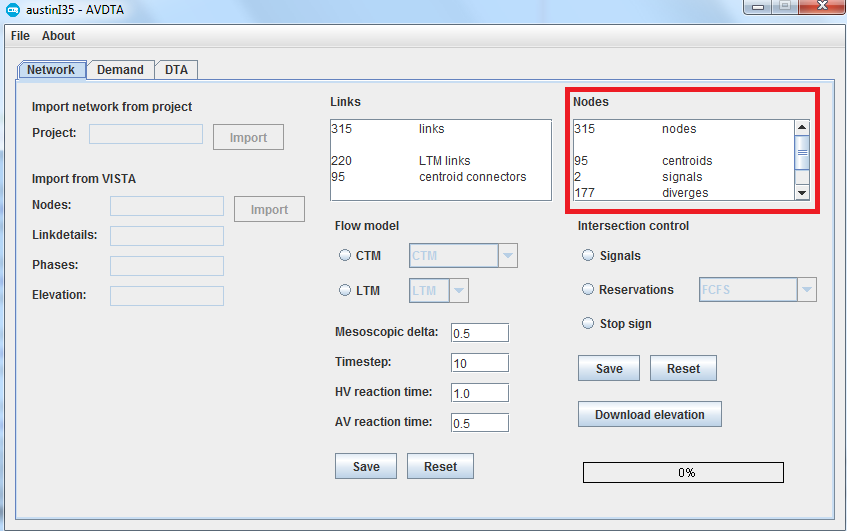
\includegraphics[width=0.8\textwidth]{images/nodes1.png}
\end{center}

The next panel controls intersections. Selecting an intersection control, then pressing the ``save'' button, will result in all intersections converted to the specified intersection control.
\begin{center}
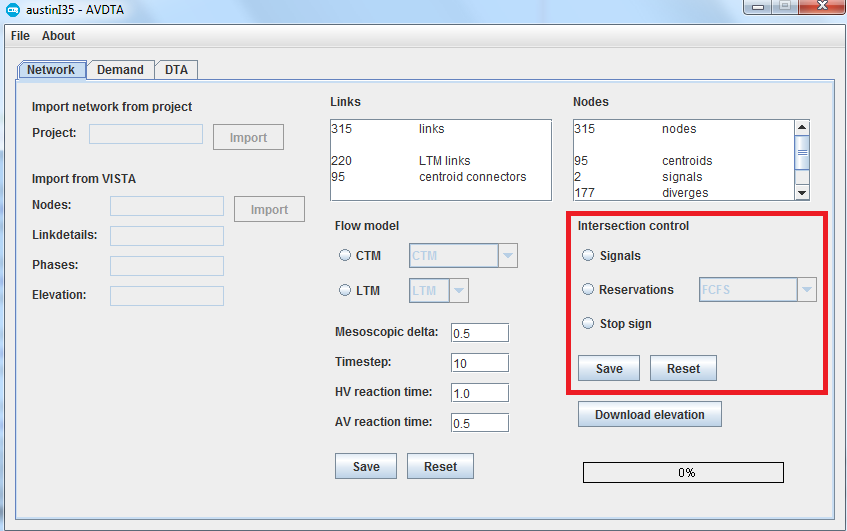
\includegraphics[width=0.8\textwidth]{images/nodes2.png}
\end{center}

The final panel will attempt to download elevation data from the Google Maps API. This will only affect nodes for which the elevation is 0. This requires a connection to the internet. The download may take some time because a delay between requests is necessary to avoid being rejected as a DOS attack. In addition, the Google Maps API may limit the number of requests per day. If the process exits with an error, restart it later. It will save progress and continue from where it left off.
\begin{center}
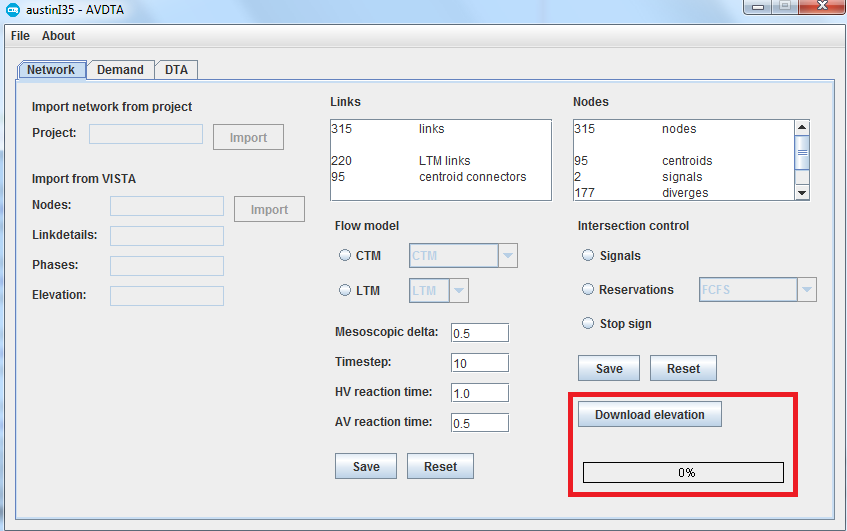
\includegraphics[width=0.8\textwidth]{images/nodes3.png}
\end{center}





\section{Links}
\label{sec:links}

\subsection{\texttt{links.txt}}

Each line in the \texttt{links.txt} file corresponds to a link in the network. The \texttt{links.txt} file has columns
\begin{center}
\begin{tabular}{ccccccccc}
\hline
id & type & source & dest & length & ffspd & w & capacity & num\_lanes \\\hline
\end{tabular}
\end{center}
\paragraph*{id} The id of the link. Each link must have an unique, positive id, but the ids do not have to be consecutive.
\paragraph*{type} This determines the flow model used for the link. The possible types are
\begin{center}
\begin{tabular}{lcl}
\hline Flow model & Type & Description\\\hline
CTM & 100 & Multiclass CTM~\cite{levin2016multiclass} \\
& 102 & CTM with DLR~\cite{levin2016cell}\\
& 103 & CTM with shared transit lane\\\hline
LTM & 200 & Standard LTM~\cite{yperman2005link, yperman2007link}\\
& 205 & LTM with CACC\\\hline
Centroid connector & 1000 & Link between a centroid and a node\\\hline
\end{tabular}
\end{center}
Standard CTM is achieved through type 100 with HVs.
\paragraph*{source} The id of the source node.
\paragraph*{dest} The id of the destination node.
\paragraph*{length} The length of the link, in feet. 
\paragraph*{ffspd} The free flow speed of the link, in miles per hour. Note that the free flow travel time is rounded up to the nearest time step.
\paragraph*{w} The congested wave speed of the link, in miles per hour. For LTM links, the free flow speed, capacity, and congested wave speed must be consistent as the fundamental diagram is over-determined. This is not an issue with CTM because CTM accepts a trapezoidal fundamental diagram. A typical value is half of the free flow speed.
\paragraph*{capacity} The capacity \textit{per lane} for the link, in vehicles per hour.
\paragraph*{num\_lanes} The number of lanes on the link. This affects the total capacity as well as intersection dynamics.

Note that for centroid connectors, the free flow travel time does not depend on the length and free flow speed, but is a constant 1 time step. Also, centroid connectors are not restricted by wavespeed or capacity limitations. 

With CTM, the minimum number of cells per link is two. This means the minimum free flow travel time is two time steps.

\subsection{GUI}

The center panel of the ``networks'' tab is used to interact with links. The uppermost text area displays information about the network, including the number of total links, and the number of links of various types.
\begin{center}
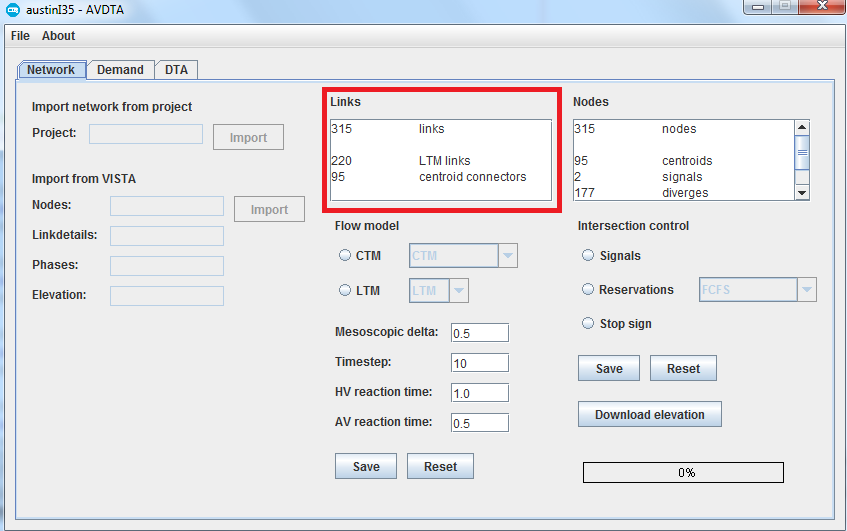
\includegraphics[width=0.8\textwidth]{images/links1.png}
\end{center}

The lower panel provides an interface for modifying the link flow model and network options. Selecting the ``CTM'' or ``LTM'' radio buttons, then pressing ``save'', will change all non-centroid connector links to the selected type. The ``mesoscopic delta'' field will set the congested wave speed to the specified fraction of the free flow speed for each link. The remaining text fields are network options (Section \ref{sec:options}).
\begin{center}
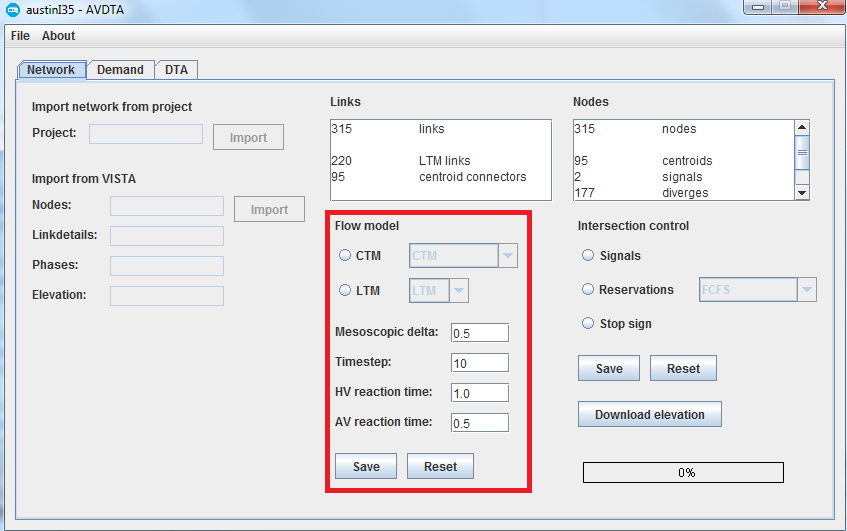
\includegraphics[width=0.8\textwidth]{images/links2.png}
\end{center}


\section{Import network}

The left hand side of the ``network tab'' contains an interface to import data from other sources. Note that using this interface will overwrite the network data of the project. There are two options. First, the network can be imported from any AVDTA project. This includes DTA projects and projects of other types. 
\begin{center}
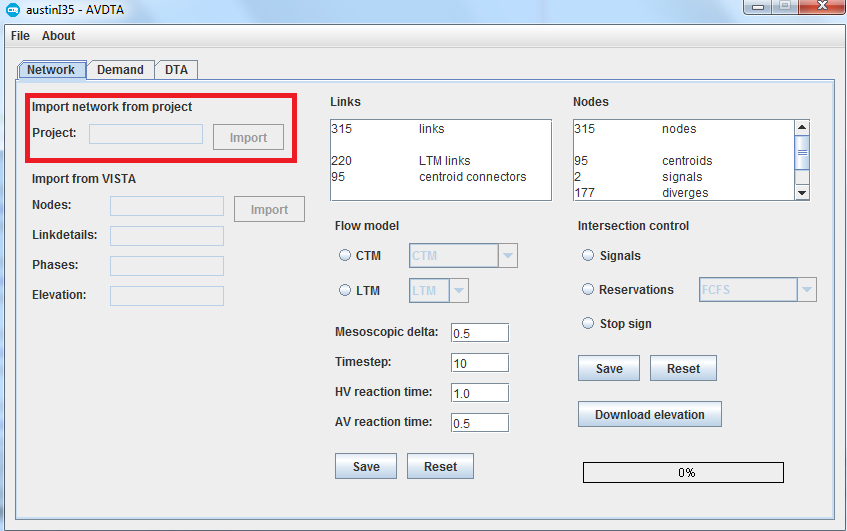
\includegraphics[width=0.8\textwidth]{images/network1.png}
\end{center}
Click on the text field to select a project file.

The second option is to import from VISTA. Copy the \texttt{nodes}, \texttt{linkdetails}, \texttt{phases}, and \texttt{signals} tables into text files, and select them by clicking on the text field. An optional elevation file can be used to fill node elevations. It is not required to import the network; if left blank, elevations of 0 will be used.
\begin{center}
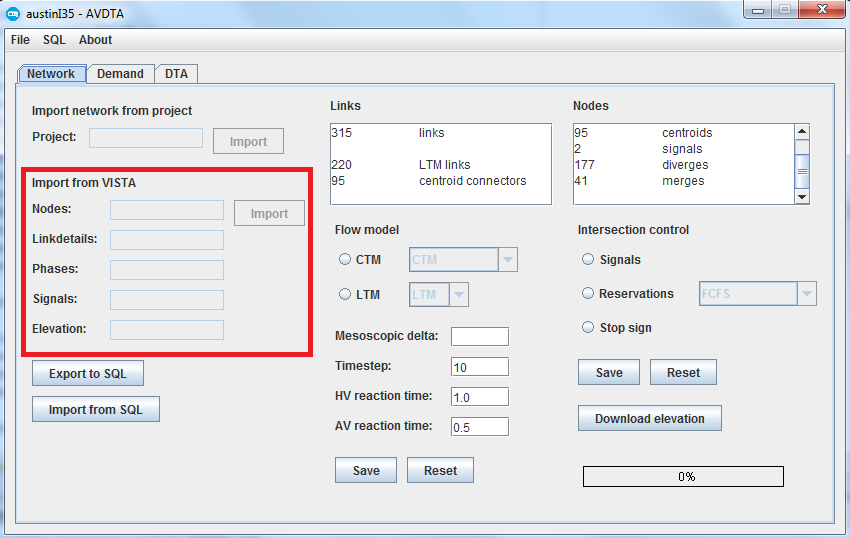
\includegraphics[width=0.8\textwidth]{images/network2.png}
\end{center}
AVDTA and VISTA use different file formats, so it is not recommended to copy VISTA tables into AVDTA directly.

The third option is to export or import data to/from SQL. This allows data to be manipulated within SQL, then returned to AVDTA in the appropriate format. To use SQL, the connection must first be set up (Section \ref{sec:setupsql}). Exporting will create and populate \texttt{nodes}, \texttt{linkdetails}, \texttt{phases}, \texttt{signals}, and \texttt{options} tables in the SQL database. Importing will copy the contents of these tables into AVDTA.
\begin{center}
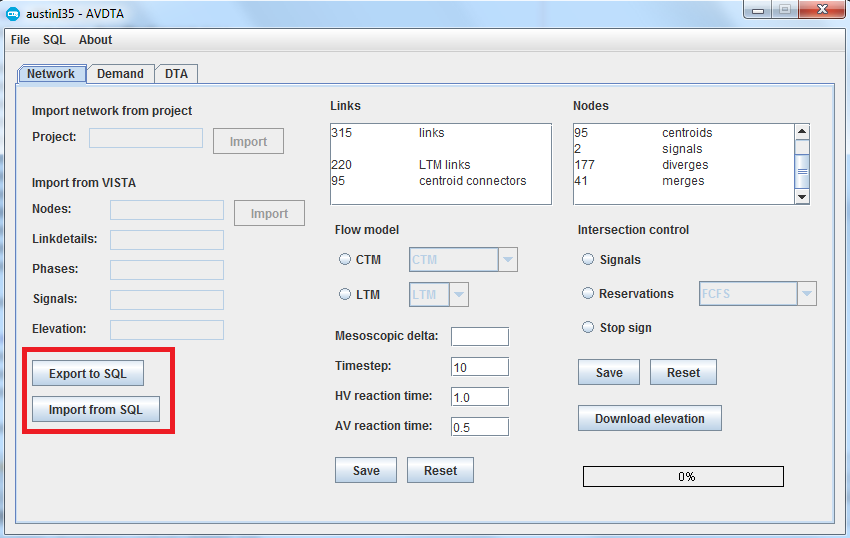
\includegraphics[width=0.8\textwidth]{images/sql2.png}
\end{center}
